\documentclass[11pt]{article}

% ============================================================
%  Packages
% ============================================================
\usepackage[utf8]{inputenc}
\usepackage[T1]{fontenc}
\usepackage{lmodern}
\usepackage[margin=1in]{geometry}

% Math
\usepackage{amsmath,amssymb,amsfonts,amsthm}

% Tables
\usepackage{booktabs}
\usepackage{array}

% Figures
\usepackage{graphicx}
\usepackage{tikz}
\usetikzlibrary{arrows.meta,positioning,shapes.geometric,fit}

% Colors
\usepackage[dvipsnames]{xcolor}

% Bibliography
\usepackage[numbers,sort&compress]{natbib}

% Hyperlinks
\usepackage[colorlinks=true,linkcolor=MidnightBlue,citecolor=OliveGreen,urlcolor=BrickRed]{hyperref}

% Misc
\usepackage{enumitem}
\usepackage{microtype}
\usepackage{url}
\usepackage{xspace}

% ============================================================
%  Theorem environments
% ============================================================
\newtheorem{definition}{Definition}[section]
\newtheorem{axiom}{Axiom}[section]
\newtheorem{proposition}{Proposition}[section]
\newtheorem{theorem}{Theorem}[section]
\newtheorem{corollary}{Corollary}[section]
\newtheorem{example}{Example}[section]

% ============================================================
%  Macros
% ============================================================
\newcommand{\DL}{\ensuremath{\mathcal{SHOIQ}}\xspace}
\newcommand{\TBox}{\ensuremath{\mathcal{T}}\xspace}
\newcommand{\ABox}{\ensuremath{\mathcal{A}}\xspace}
\newcommand{\KB}{\ensuremath{\mathcal{K}}\xspace}
\newcommand{\sqsub}{\sqsubseteq}
\DeclareMathOperator*{\bigsqcap}{\sqcap}

% ============================================================
%  Title
% ============================================================
\title{%
  From Ontology-Controlled Systems \\
  to Oversight-Controlled Training: \\
  Formal Foundations for Human--LLM \\
  Alignment Signal Validation%
}

\author{
  Vladimir Ovcharov\thanks{Correspondence: \texttt{volodymyr@legal.org.ua}}\\[4pt]
  LEX AI LLC, Kyiv, Ukraine\\
}

\date{2026}

\begin{document}
\maketitle

% ============================================================
%  Abstract
% ============================================================
\begin{abstract}
Ontology-based filtering of human oversight signal predicts downstream outcome quality: on 30{,}510 edit-traces from a production legal AI platform, sessions classified as full oversight by a formal domain constitution exhibit a 3--6$\times$ higher rejection rate than partial-oversight sessions, concentrating the most informative alignment action---binary halt of agentic trajectories, which correlates with 78\% positive outcomes.
This finding bridges two previously disjoint research programs: ontology-controlled systems~\citep{palagin2006architecture, palagin2023ontochatgpt}, which govern system output via formal structure, and LLM alignment, which lacks formal criteria for distinguishing valid human corrections from noise.

We formalize a \emph{domain constitution}---five axiomatically defined, provably independent conditions in \DL description logic---under which human edit-traces on agentic LLM output constitute valid training signal for RLHF.
The formalization is implemented as an OWL~2~DL ontology: given workflow metadata as ABox assertions, a standard reasoner (HermiT, Pellet) classifies each session as full, partial, or invalid oversight in sub-second time.
We show that ontological control of human oversight ($\mathsf{ValidOversight}$) is a strict specialization of ontological control of system output ($\mathsf{OntoChatGPT\_Control}$): the two operate on complementary levels of the same conceptual stack, and their integration is satisfiable.
Among the five conditions, information asymmetry (C4) is identified as the critical evolutionary vulnerability---the only condition whose satisfiability depends on agent capability, connecting the formalization to the scalable oversight research program~\citep{bowman2022measuring}.
\end{abstract}

\noindent\textbf{Keywords:} ontology-controlled systems, domain constitution, description logic, RLHF, alignment, edit-trace oversight, OWL, human oversight, LLM

% ============================================================
\section{Introduction}
\label{sec:intro}
% ============================================================

% --------------------------------------------------------
\subsection{The Problem: Preference Signal Without Formal Validity Criteria}
\label{sec:problem}
% --------------------------------------------------------

Reinforcement learning from human feedback (RLHF) has become the dominant paradigm for aligning large language models with human intent~\citep{christiano2017deep, ouyang2022training}.
The paradigm rests on a simple premise: human judgments about model outputs---expressed as preference labels, rankings, or corrections---provide a training signal that steers the model toward desirable behavior.
Direct Preference Optimization (DPO)~\citep{rafailov2023direct} simplified the training pipeline by eliminating the intermediate reward model, but the upstream question remains unchanged: \emph{which human judgments constitute valid training signal?}

Current practice treats this question as unproblematic.
Crowd workers on Amazon Mechanical Turk rate pairs of model outputs~\citep{ouyang2022training}.
Expert annotators evaluate in controlled settings~\citep{bai2022constitutional}.
AI models generate synthetic preferences via self-evaluation (RLAIF)~\citep{lee2023rlaif}.
In each case, the implicit assumption is that any preference label, from any context, is equally valid as training data.
There are no formal criteria---no axioms, no decidable conditions, no automated verification---for distinguishing valid preference signal from noise.

This absence of formal validity criteria would be unremarkable if the signal sources were homogeneous.
But they are not.
A crowd worker rating two completions in a web interface and a domain expert correcting an LLM agent's output within a production workflow occupy fundamentally different epistemic positions.
The crowd worker operates without persistent state, without compositional context, without production consequences.
The domain expert operates with all three.
Treating their annotations as interchangeable discards information about signal quality that is, in principle, formalizable.

% --------------------------------------------------------
\subsection{An Empirical Observation}
\label{sec:observation}
% --------------------------------------------------------

\citet{ovcharov2026edittrace} documented an empirical case that sharpens this problem.
A single practitioner shipped 1{,}547 merged pull requests across 7 production repositories in 105 days using an LLM agent (Claude Code) as the primary engineering counterpart---building a legal AI platform (Legal.org.ua) with 70+ MCP tools, 380M+ records in the data pipeline, and paying customers.
Validated outcomes included acceptance by Google for Startups, NVIDIA Inception, and AWS Activate.

Every human correction on the agent's output was captured as an edit-trace: the agent's proposed output, the human's corrected version, and the downstream outcome of the corrected artifact.
The resulting dataset---30{,}510 edit pairs across 2{,}892 sessions, with 1{,}579 attributed outcomes---exhibited a qualitatively different distribution from what detached annotation would produce: 80.7\% of all corrections were substantive rewrites (median normalized edit distance: 0.84), and binary rejection of agent output correlated with 78\% positive downstream outcomes.

The paper proposed five informal conditions---termed a ``domain constitution''---under which these edit-traces constitute valid oversight signal rather than noise.
The conditions were stated in structured English, motivated by empirical observation, and validated statistically.
But they were not \emph{formalized}: they lacked the precision of description logic axioms, the decidability of automated reasoning, and the implementability of an OWL ontology.

% --------------------------------------------------------
\subsection{The Ontological Control Principle}
\label{sec:principle}
% --------------------------------------------------------

The formalization gap identified above has a natural solution in a research tradition developed over the past two decades at the V.M.~Glushkov Institute of Cybernetics, NAS of Ukraine.

\citet{palagin2006architecture} introduced the principle of \emph{ontology-controlled systems}: formal ontological structure should not merely describe a system but actively \emph{control} its behavior.
This principle has been applied at progressively higher levels of the computational stack---from system architecture~\citep{palagin2006architecture} to NL text processing~\citep{palagin2012knowledge, palagin2020distributional} to LLM output generation~\citep{palagin2023ontochatgpt, palagin2024neural} to evolutionary system dynamics~\citep{palagin2025evolutionary}---with consistent results: formal structure, when used as a control mechanism rather than passive metadata, improves both the quality and verifiability of system behavior.

The present work extends this principle to one additional level.
If formal ontological structure can control what an LLM produces (as demonstrated by OntoChatGPT), can it also control which human corrections on LLM output are valid training signal?

We argue that it can, and we formalize this argument.

% --------------------------------------------------------
\subsection{Contributions}
\label{sec:contributions}
% --------------------------------------------------------

This paper makes four contributions:

\begin{enumerate}[label=(\arabic*),leftmargin=2em]

\item \textbf{Formalization of the domain constitution in \DL description logic} (Section~\ref{sec:formal}).
The five informal conditions from~\citet{ovcharov2026edittrace} are expressed as general concept inclusions (GCIs) in \DL, with a defined concept $\mathsf{ValidOversight}$ that is the conjunction of all five.
We prove three formal properties: decidability of instance classification, independence of the five conditions, and monotonicity of the oversight grade under assertion growth.

\item \textbf{Formal comparison of output-level and oversight-level ontological control} (Section~\ref{sec:comparison}).
We analyze the relationship between OntoChatGPT~\citep{palagin2023ontochatgpt} and the domain constitution via subsumption queries, showing that $\mathsf{ValidOversight}$ is a \emph{strict specialization} of $\mathsf{OntoChatGPT\_Control}$: every valid oversight instance satisfies the conditions that define ontology-controlled output, but not conversely.
This formally confirms that edit-trace oversight \emph{extends} the ontology-controlled paradigm rather than replacing it.

\item \textbf{OWL~2~DL ontology for automated oversight classification} (Section~\ref{sec:owl}).
The TBox is implemented as an OWL ontology with automated reasoning via HermiT~\citep{shearer2008hermit}.
Workflow instances from the LEX~AI case study are instantiated as ABox individuals and automatically classified as full, partial, or invalid oversight.

\item \textbf{Empirical validation of ontology-based signal filtering} (Section~\ref{sec:empirical}).
We demonstrate that edit-traces from workflows classified as $\mathsf{ValidOversight}$ correlate with better downstream outcomes than unfiltered traces, providing empirical support for the claim that formal filtering of preference data improves training signal quality.

\end{enumerate}

% --------------------------------------------------------
\subsection{Structure of the Paper}
\label{sec:structure}
% --------------------------------------------------------

Section~\ref{sec:evolution} traces the evolution of the ontological control principle across five levels, from system architecture (2006) to human oversight validation (this paper).
Section~\ref{sec:formal} presents the formal model: signature, TBox axiomatization, defined concepts, negative classification, graded oversight, reasoning tasks, and formal properties.
Section~\ref{sec:comparison} compares OntoChatGPT and the domain constitution: shared principle, structural differences, subsumption analysis, and integration architecture.
Section~\ref{sec:owl} describes the OWL~2~DL implementation and automated verification on the LEX~AI case study.
Section~\ref{sec:empirical} provides empirical validation.
Section~\ref{sec:discussion} discusses implications for RLHF methodology and the role of evolutionary cybernetics in analyzing oversight dynamics.
Section~\ref{sec:conclusion} concludes.


% ============================================================
\section{Evolution of Ontological Control}
\label{sec:evolution}
% ============================================================

The principle that formal ontological structure should \emph{control} system behavior---not merely describe or annotate it---has evolved through four successive levels of abstraction over the past two decades.
Each level retains the core invariant (a formal structure governs a computational process) while shifting the \emph{object of control} from hardware architecture to natural language processing to LLM output generation.
This paper proposes a fifth level: ontological control over the process by which human oversight of LLM output is validated as training signal.

Table~\ref{tab:evolution} summarizes the progression.

\begin{table}[h]
\centering
\caption{Evolution of ontological control: what the formal structure governs at each level.}
\label{tab:evolution}
\begin{tabular}{@{}clll@{}}
\toprule
\textbf{Level} & \textbf{Period} & \textbf{Object of control} & \textbf{Key reference} \\
\midrule
I   & 2003--2006 & System architecture        & \citet{palagin2006architecture} \\
II  & 2012--2020 & NL text processing pipeline & \citet{palagin2012knowledge,palagin2020distributional} \\
III & 2023--2024 & LLM output generation       & \citet{palagin2023ontochatgpt,palagin2024neural} \\
IV  & 2025       & Evolutionary system dynamics & \citet{palagin2025evolutionary} \\
V   & 2026       & Human oversight validation   & This paper \\
\bottomrule
\end{tabular}
\end{table}

% --------------------------------------------------------
\subsection{Level I: Ontological Control of System Architecture (2003--2006)}
\label{sec:level1}
% --------------------------------------------------------

\citet{palagin2006architecture} introduced the foundational distinction: an ontology in a computer system can serve as passive metadata (a catalog of concepts and relations) or as an active \emph{control mechanism} that governs the system's runtime behavior.
The paper argued for the latter interpretation: the ontology defines not only what the system knows but what it \emph{does}---which modules are instantiated, how data flows between them, what processing strategies are selected.

This was a departure from the contemporaneous use of ontologies in the Semantic Web community, where OWL ontologies primarily served as interoperability schemas~\citep{grau2008owl2}.
In Palagin's formulation, the ontology occupies the role that a control program occupies in classical von Neumann architecture: it is the structure that determines execution.

The key insight for the present work is the \emph{generality} of this principle.
If formal structure can control system architecture, the question arises: what \emph{else} can it control?
The subsequent two decades provide an empirical answer: progressively higher levels of the computational stack.

% --------------------------------------------------------
\subsection{Level II: Ontological Control of NL Text Processing (2012--2020)}
\label{sec:level2}
% --------------------------------------------------------

The second level applies ontological control to natural language processing pipelines.
\citet{palagin2012knowledge} developed methods for ontology-driven extraction of knowledge from natural language texts, where the domain ontology governs which entities are recognized, what relations are extracted, and how extracted knowledge is represented in formal-logical form.
The ontology does not merely label the output of an NLP pipeline---it \emph{controls} which pipeline stages execute and what constitutes a valid extraction result.

\citet{palagin2020distributional} extended this principle to distributional semantics.
The Semantic Pre-processing Technology (SPT) pipeline uses ontological structure as an \emph{anchor} for learning distributed term representations.
Where standard word embedding methods (Word2Vec, GloVe) learn representations from co-occurrence statistics alone, SPT uses the domain ontology to:
(a)~define term boundaries (transitioning from word-level to term-level embeddings),
(b)~constrain the embedding space so that ontologically related terms cluster appropriately, and
(c)~provide terminological supervision that reduces the data requirements for domain-specific embedding training.

The relevance to the present work is twofold.
First, the SPT pipeline demonstrates that domain-specific formal structure improves representation learning---a principle we argue extends to preference learning (Section~\ref{sec:empirical}).
Second, the ontology-anchored embedding approach is directly applicable to the legal AI domain where our edit-traces originate: 100.5 million Ukrainian court decisions constitute a corpus where morphological complexity (Ukrainian is a highly inflectional language with seven cases and three genders) makes ontological anchoring especially valuable.

% --------------------------------------------------------
\subsection{Level III: Ontological Control of LLM Output (2023--2024)}
\label{sec:level3}
% --------------------------------------------------------

The emergence of large language models created a new control surface: the model's generation process.
\citet{palagin2023ontochatgpt} developed OntoChatGPT, a system where a formal OWL ontology generates structured prompts that control ChatGPT's output.
The mechanism is a two-stage pipeline:

\begin{enumerate}[nosep]
  \item A \emph{meta-ontology} encodes domain knowledge (concepts, relations, constraints, expected output structures) in OWL format.
  \item At inference time, the meta-ontology is traversed to generate \emph{structured prompts} that instruct the LLM to produce output conforming to the ontological structure.
\end{enumerate}

This is ontological control in the strict sense: the OWL ontology does not describe what the LLM might produce---it \emph{governs} what it does produce.
The system was demonstrated in the medical rehabilitation domain (Ukrainian language), where ontology-driven prompts produced contextually relevant and structurally consistent responses~\citep{palagin2023ontochatgpt}.

\citet{palagin2024neural} generalized this into a methodological framework: the ``integrated use of neural network and ontolinguistic paradigms.''
The key argument is that neither the neural paradigm (statistical learning from data) nor the ontolinguistic paradigm (formal knowledge representation) is sufficient alone for complex NLP tasks.
The neural paradigm learns patterns but lacks formal structure; the ontolinguistic paradigm provides structure but lacks the ability to generalize from data.
Integration---using ontological structure to guide neural learning---produces results superior to either paradigm in isolation.

In parallel, \citet{palagin2023dialogue} applied ontological control to dialogue systems: an OWL ontology is automatically constructed from unstructured text, converted to a Neo4j graph database, and then used to govern dialogue responses via formal Cypher queries.
The dialogue system does not generate free-form responses; it produces responses that are \emph{derivable} from the ontological graph.

These Level~III systems share a critical property: the ontology controls \textbf{what the model produces at inference time}.
The formal structure operates on the \emph{output} of the system.
This is effective for improving the quality and consistency of individual LLM outputs, but it does not address a different question: how to improve the \emph{training signal} that shapes the model's future behavior.

% --------------------------------------------------------
\subsection{Level IV: Ontological Control of Evolutionary Dynamics (2025)}
\label{sec:level4}
% --------------------------------------------------------

The most recent extension~\citep{palagin2025evolutionary} moves ontological control from static system architectures to \emph{evolving} systems where goals, constraints, and structures themselves change over time.
Evolutionary cybernetics, as formalized in this work, addresses systems where the classical control-theoretic assumption of a fixed objective function does not hold.
Instead, the system's objectives, the constraints it operates under, and its structural organization co-evolve with its environment.

This level is directly relevant to the human--LLM oversight regime documented in~\citet{ovcharov2026edittrace}.
The practitioner-agent composition observed there---where neither the human nor the agent achieves the observed output independently---is not a static equilibrium.
As the agent's capabilities improve through training (including training on the very edit-traces the practitioner generates), the nature of oversight changes: corrections may become more targeted and architecturally informed, the information asymmetry (Condition~C4) may shift, and the domain constitution itself may require revision.

\citet{palagin2025evolutionary} provides the theoretical vocabulary for analyzing this dynamic: the domain constitution is not a fixed control program but an \emph{evolutionary constraint} that co-evolves with the system it governs.
Whether the practitioner-agent equilibrium is stable under further capability scaling~\citep{burns2023weak} is an instance of the broader question evolutionary cybernetics poses: under what conditions do co-evolving control structures maintain their functional role?

% --------------------------------------------------------
\subsection{Level V: Ontological Control of Human Oversight (This Paper)}
\label{sec:level5}
% --------------------------------------------------------

We propose that the same principle---formal structure controls behavior---applies to one additional level: the process by which human oversight of LLM output is validated as training signal for model improvement.

The motivation arises from a structural gap in the RLHF literature~\citep{christiano2017deep, ouyang2022training}.
Current methods collect human preferences via crowd annotation~\citep{ouyang2022training}, AI self-evaluation~\citep{bai2022constitutional, lee2023rlaif}, or expert rating.
None of these methods provides \emph{formal criteria} for when a human correction constitutes valid training signal versus noise.
The implicit assumption is that any human preference label, from any context, is equally valid as training data.

\citet{ovcharov2026edittrace} challenged this assumption empirically.
When a practitioner works recursively with an LLM agent over production workflows (1{,}547 merged PRs, 105 days, 7 repositories), the resulting edit-traces exhibit a qualitatively different distribution from what detached annotation would produce: 80.7\% substantive rewrites (median normalized edit distance 0.84), with binary rejection correlating with 78\% positive downstream outcomes.
The paper proposed five informal conditions (``domain constitution'') under which these edit-traces constitute valid oversight signal.

The present work formalizes these conditions.
Table~\ref{tab:levels} shows the structural parallel across all five levels.

\begin{table}[h]
\centering
\caption{The ontological control principle across five levels of abstraction.}
\label{tab:levels}
\begin{tabular}{@{}cp{3.5cm}p{3.5cm}p{3.5cm}@{}}
\toprule
\textbf{Level} & \textbf{Formal structure} & \textbf{Controls} & \textbf{Object of control} \\
\midrule
I   & Domain ontology          & System architecture     & Which modules execute \\
II  & SPT + ontology           & NLP pipeline            & Which entities/terms are extracted \\
III & Meta-ontology (OWL)      & LLM output              & What the model generates \\
IV  & Evolutionary constraints & System dynamics          & How goals/structure co-evolve \\
V   & Domain constitution      & Oversight validation     & When human corrections are valid training signal \\
\bottomrule
\end{tabular}
\end{table}

The transition from Level~III to Level~V is the central contribution.
At Level~III, formal structure governs what the LLM produces (inference-time control).
At Level~V, formal structure governs how we determine whether human corrections on LLM output constitute valid data for improving the LLM (training-time control).
The shift is from controlling the model's \emph{generation} process to controlling the \emph{oversight} process that yields preference data for model improvement.

This is not merely a change in application domain.
It represents a change in the \emph{kind} of process being controlled.
Levels~I--III control computational processes (architecture configuration, text processing, token generation).
Level~V controls a \emph{socio-technical} process: the interaction between a human overseer and an AI system, and the conditions under which that interaction produces signal suitable for machine learning.

The formalization of this control in \DL description logic is the subject of Section~\ref{sec:formal}.


% ============================================================
\section{Formal Model of the Domain Constitution}
\label{sec:formal}
% ============================================================

We formalize the domain constitution---the set of conditions under which human corrections on LLM-agentic output constitute valid oversight signal---in \DL description logic~\citep{baader2003description}.
\DL extends $\mathcal{ALC}$ with transitive roles ($\mathcal{S}$), role hierarchies ($\mathcal{H}$), nominals ($\mathcal{O}$), inverse roles ($\mathcal{I}$), and qualified number restrictions ($\mathcal{Q}$), corresponding to the OWL~2~DL profile~\citep{grau2008owl2}.

% --------------------------------------------------------
\subsection{Signature}
\label{sec:signature}
% --------------------------------------------------------

\begin{definition}[Oversight Signature]
\label{def:signature}
The oversight signature $\Sigma_{\mathrm{ov}}$ consists of:

\medskip\noindent
\textbf{Concept names} $N_C$:
\begin{center}
\begin{tabular}{@{}ll@{}}
\toprule
\textbf{Concept} & \textbf{Intuition} \\
\midrule
$\mathsf{Agent}$         & LLM-based agentic system \\
$\mathsf{Human}$         & Practitioner performing oversight \\
$\mathsf{Session}$       & Bounded unit of human--agent interaction \\
$\mathsf{Workflow}$      & Bounded sequence of related sessions \\
$\mathsf{Artifact}$      & Output produced by $\mathsf{Agent}$ within a $\mathsf{Session}$ \\
$\mathsf{Edit}$          & Human correction applied to an $\mathsf{Artifact}$ \\
$\mathsf{Outcome}$       & Deployed result with measurable consequences \\
$\mathsf{State}$         & Persistent shared computational state \\
$\mathsf{Information}$   & Knowledge or context available to a participant \\
$\mathsf{SuccessCriterion}$ & Observable predicate defining task completion \\
$\mathsf{ProductionMetric}$ & Measurable system-level quantity \\
\bottomrule
\end{tabular}
\end{center}

\medskip\noindent
\textbf{Role names} $N_R$:
\begin{center}
\begin{tabular}{@{}lll@{}}
\toprule
\textbf{Role} & \textbf{Domain $\to$ Range} & \textbf{Properties} \\
\midrule
$\mathsf{operatesOn}$      & $\mathsf{Agent} \to \mathsf{State}$          & --- \\
$\mathsf{accessesState}$   & $\mathsf{Human} \to \mathsf{State}$          & --- \\
$\mathsf{hasState}$        & $\mathsf{Session} \to \mathsf{State}$        & --- \\
$\mathsf{hasSession}$      & $\mathsf{Workflow} \to \mathsf{Session}$     & --- \\
$\mathsf{hasArtifact}$     & $\mathsf{Session} \to \mathsf{Artifact}$     & --- \\
$\mathsf{producesArtifact}$& $\mathsf{Session} \to \mathsf{Artifact}$     & --- \\
$\mathsf{hasEdit}$         & $\mathsf{Artifact} \to \mathsf{Edit}$        & --- \\
$\mathsf{hasOutcome}$      & $\mathsf{Session} \to \mathsf{Outcome}$      & --- \\
$\mathsf{dependsOn}$       & $\mathsf{Session} \to \mathsf{Session}$      & transitive \\
$\mathsf{basedOn}$         & $\mathsf{Edit} \to \mathsf{Information}$     & --- \\
$\mathsf{accessibleTo}$    & $\mathsf{Information} \to \mathsf{Agent}$    & --- \\
$\mathsf{hasCriterion}$    & $\mathsf{Session} \to \mathsf{SuccessCriterion}$ & --- \\
$\mathsf{measuredBy}$      & $\mathsf{SuccessCriterion} \to \mathsf{ProductionMetric}$ & --- \\
$\mathsf{hasConsequence}$  & $\mathsf{Outcome} \to \mathsf{ProductionMetric}$ & --- \\
$\mathsf{partOf}$          & $\mathsf{Session} \to \mathsf{Workflow}$     & --- \\
\bottomrule
\end{tabular}
\end{center}

\medskip\noindent
\textbf{Derived concepts} (defined via role restrictions):
\begin{align}
  \mathsf{PersistentState} &\equiv \mathsf{State} \sqcap
    \exists\mathsf{operatesOn}^{-}.\mathsf{Agent} \sqcap
    \exists\mathsf{accessesState}^{-}.\mathsf{Human}
    \label{eq:persistent-state} \\[4pt]
  \mathsf{PrivateInfo} &\equiv \mathsf{Information} \sqcap
    \neg\exists\mathsf{accessibleTo}.\mathsf{Agent}
    \label{eq:private-info} \\[4pt]
  \mathsf{GroundedCriterion} &\equiv \mathsf{SuccessCriterion} \sqcap
    \exists\mathsf{measuredBy}.\mathsf{ProductionMetric}
    \label{eq:grounded-criterion} \\[4pt]
  \mathsf{ConsequentialOutcome} &\equiv \mathsf{Outcome} \sqcap
    \exists\mathsf{hasConsequence}.\mathsf{ProductionMetric}
    \label{eq:consequential-outcome}
\end{align}
\end{definition}

% --------------------------------------------------------
\subsection{TBox: Axiomatization of the Five Conditions}
\label{sec:tbox}
% --------------------------------------------------------

The domain constitution is a TBox \TBox consisting of five general concept inclusions (GCIs), each capturing one necessary condition for valid oversight.
$\mathsf{ValidOversight}$ is a \emph{defined concept}---an individual (workflow instance) is classified as valid oversight if and only if it satisfies all five conditions simultaneously.

\begin{axiom}[C1: Shared Persistent State]
\label{ax:c1}
Valid oversight requires that the agent and the human operate on a shared, persistent state---a computational environment (codebase, file system, version history) that accumulates changes across sessions and is accessible to both participants.
\begin{equation}
  \mathsf{ValidOversight} \sqsub
    \exists\mathsf{hasState}.\mathsf{PersistentState}
  \label{eq:c1}
\end{equation}
where $\mathsf{PersistentState}$ is defined as in~(\ref{eq:persistent-state}).
A workflow operating on isolated, ephemeral snippets without shared state fails C1.

\medskip\noindent
\emph{Rationale.}
Without persistent shared state, human corrections are context-free: they reflect preferences over isolated outputs rather than oversight over an evolving system.
Persistent state ensures each correction is informed by the cumulative history of prior agent behavior and its consequences~\citep{ovcharov2026edittrace}.
\end{axiom}

\begin{axiom}[C2: Compositional Task Layering]
\label{ax:c2}
Valid oversight requires that sessions compose into dependency chains: the output of one session serves as input context for subsequent sessions.
\begin{equation}
  \mathsf{ValidOversight} \sqsub
    \exists\mathsf{partOf}.\left(
      \mathsf{Workflow} \sqcap
      \exists\mathsf{hasSession}.\left(
        \mathsf{Session} \sqcap \exists\mathsf{dependsOn}.\mathsf{Session}
      \right)
    \right)
  \label{eq:c2}
\end{equation}
The role $\mathsf{dependsOn}$ is declared transitive:
\begin{equation}
  \mathsf{Trans}(\mathsf{dependsOn})
  \label{eq:c2-trans}
\end{equation}
This enables reasoning over multi-hop compositional chains: if session $s_3$ depends on $s_2$ and $s_2$ depends on $s_1$, then $s_3$ is compositionally linked to $s_1$.

\medskip\noindent
\emph{Rationale.}
Single-turn corrections cannot capture compositional failure modes---cases where each individual output appears adequate but the composition fails.
An edit correcting an architectural decision that conflicts with a decision made weeks earlier encodes long-range dependency information that no single-turn annotation scheme captures.
\end{axiom}

\begin{axiom}[C3: Grounding in Observable Reality]
\label{ax:c3}
Valid oversight requires that success criteria are defined as predicates over observable production metrics, not subjective preferences.
\begin{equation}
  \mathsf{ValidOversight} \sqsub
    \exists\mathsf{hasCriterion}.\mathsf{GroundedCriterion}
  \label{eq:c3}
\end{equation}
where $\mathsf{GroundedCriterion}$ is defined as in~(\ref{eq:grounded-criterion}).

\medskip\noindent
\emph{Rationale.}
Oversight that rests on subjective preference alone is indistinguishable from taste.
Corrections grounded in observable system behavior---a deployment failure, a latency spike, an error rate increase---encode causal information about what works and what does not.
\end{axiom}

\begin{axiom}[C4: Information Asymmetry Favoring the Human]
\label{ax:c4}
Valid oversight requires that at least some human corrections are based on information not accessible to the agent.
\begin{equation}
  \mathsf{ValidOversight} \sqsub
    \exists\mathsf{hasArtifact}.\left(
      \mathsf{Artifact} \sqcap \exists\mathsf{hasEdit}.\left(
        \mathsf{Edit} \sqcap \exists\mathsf{basedOn}.\mathsf{PrivateInfo}
      \right)
    \right)
  \label{eq:c4}
\end{equation}
where $\mathsf{PrivateInfo}$ is defined as in~(\ref{eq:private-info}).

\medskip\noindent
\emph{Rationale.}
Oversight is meaningful precisely because the overseer holds information the overseen system lacks: business priorities, regulatory requirements, user feedback, personal stake in outcomes.
If corrections reflect only information already available to the agent, the edit-trace is redundant with the agent's own uncertainty.
\end{axiom}

\begin{axiom}[C5: Consequential Grounding]
\label{ax:c5}
Valid oversight requires that the workflow produces outcomes with measurable real-world consequences.
\begin{equation}
  \mathsf{ValidOversight} \sqsub
    \exists\mathsf{hasOutcome}.\mathsf{ConsequentialOutcome}
  \label{eq:c5}
\end{equation}
where $\mathsf{ConsequentialOutcome}$ is defined as in~(\ref{eq:consequential-outcome}).

\medskip\noindent
\emph{Rationale.}
Oversight signal must connect to real consequences to avoid the same detachment that afflicts crowd annotation.
When corrected artifacts ship and succeed or fail in production, the edit-trace acquires outcome labels that close the loop between correction and consequence.
\end{axiom}

% --------------------------------------------------------
\subsection{Defined Concept: Valid Oversight}
\label{sec:valid-oversight}
% --------------------------------------------------------

\begin{definition}[Valid Oversight]
\label{def:valid-oversight}
The concept $\mathsf{ValidOversight}$ is the conjunction of all five axiomatic conditions:
\begin{equation}
\boxed{
  \mathsf{ValidOversight} \equiv
    \mathsf{C1} \sqcap \mathsf{C2} \sqcap \mathsf{C3} \sqcap \mathsf{C4} \sqcap \mathsf{C5}
}
\label{eq:valid-oversight}
\end{equation}
where each $\mathsf{C}_i$ is the right-hand side of the corresponding GCI~(\ref{eq:c1})--(\ref{eq:c5}).
\end{definition}

This is a \emph{necessary and sufficient} definition: an OWL~2~DL reasoner can automatically classify any workflow individual as $\mathsf{ValidOversight}$ (or not) given its asserted properties.

% --------------------------------------------------------
\subsection{Negative Classification: Invalid Oversight Patterns}
\label{sec:negative}
% --------------------------------------------------------

The domain constitution defines its negation: interaction patterns that fail one or more conditions.
These are formally derivable as non-entailments from the TBox.

\begin{proposition}[Non-entailment of invalid patterns]
\label{prop:negative}
The following workflow patterns are provably not classified as $\mathsf{ValidOversight}$:
\end{proposition}

\begin{enumerate}[label=(\alph*),leftmargin=2em]

\item \textbf{Traditional IDE with undo history (C1 only).}
Let $w_1$ be a system with persistent state across sessions (an IDE undo buffer) but no edit-trace logging of operator corrections; sessions compose into dependency chains (C2), criteria are grounded (C3), the operator holds private context (C4), and the workflow ships production artifacts (C5).
\begin{align}
  \ABox_1 &= \{ \mathsf{Workflow}(w_1),\; \mathsf{hasSession}(w_1, s),\;
               \neg\exists\mathsf{hasState}.\mathsf{PersistentState}(w_1) \} \notag \\
  \KB &= \langle \TBox, \ABox_1 \rangle \notag \\
  \KB &\not\models \mathsf{ValidOversight}(w_1) \qquad \text{(fails C1 only)}
\end{align}

\item \textbf{One-shot code generation with in-session feedback (C2 only).}
Let $w_2$ be a one-shot tool that logs operator corrections within a single session (C1 is satisfied by the session-scoped state), but has no persistent state across sessions and no compositional dependency chain; criteria are grounded (C3), the operator holds private information (C4), and an artifact is deployed (C5).
\begin{align}
  \ABox_2 &= \{ \mathsf{Workflow}(w_2),\; \mathsf{hasSession}(w_2, s),\;
               \neg\exists\mathsf{partOf}.({\mathsf{Workflow} \sqcap \exists\mathsf{hasSession}.(\mathsf{Session} \sqcap \exists\mathsf{dependsOn}.\mathsf{Session})})(w_2) \} \notag \\
  \KB &= \langle \TBox, \ABox_2 \rangle \notag \\
  \KB &\not\models \mathsf{ValidOversight}(w_2) \qquad \text{(fails C2 only)}
\end{align}

\item \textbf{Automated CI/CD pipeline.}
Let $w_3$ be a workflow where all edits are based on information accessible to the agent (test results, linter output).
\begin{align}
  \forall e \in \mathsf{Edit}(w_3)&: \; \exists i.\; \mathsf{basedOn}(e, i) \wedge \mathsf{accessibleTo}(i, a) \notag \\
  \KB &\not\models \mathsf{ValidOversight}(w_3) \qquad \text{(fails C4)}
\end{align}

\item \textbf{Tutorial or learning use.}
Let $w_4$ be a workflow with no deployed outcomes.
\begin{align}
  \neg\exists o.\; &\mathsf{hasOutcome}(w_4, o) \wedge \mathsf{ConsequentialOutcome}(o) \notag \\
  \KB &\not\models \mathsf{ValidOversight}(w_4) \qquad \text{(fails C5)}
\end{align}

\item \textbf{Pair programming without success criteria.}
Let $w_5$ be a workflow with shared state and compositional chains but no grounded success criteria.
\begin{align}
  \neg\exists c.\; &\mathsf{hasCriterion}(w_5, c) \wedge \mathsf{GroundedCriterion}(c) \notag \\
  \KB &\not\models \mathsf{ValidOversight}(w_5) \qquad \text{(fails C3)}
\end{align}

\end{enumerate}

% --------------------------------------------------------
\subsection{Partial Oversight and Graded Classification}
\label{sec:partial}
% --------------------------------------------------------

In practice, workflows may satisfy some but not all conditions.
We define a graded classification based on the number of satisfied conditions.

\begin{definition}[Oversight Grade]
\label{def:grade}
For a workflow individual $w$ and TBox \TBox, the \emph{oversight grade} $\gamma(w)$ is:
\begin{equation}
  \gamma(w) = \left| \{ i \in \{1,...,5\} : \KB \models \mathsf{C}_i(w) \} \right|
\end{equation}
We define three tiers:
\begin{align}
  \mathsf{FullOversight}    &\equiv \mathsf{ValidOversight} && (\gamma = 5) \\
  \mathsf{PartialOversight} &\equiv (\gamma \geq 3) \sqcap \neg\mathsf{ValidOversight} && (\gamma \in \{3,4\}) \\
  \mathsf{InvalidOversight} &\equiv \neg\mathsf{PartialOversight} \sqcap \neg\mathsf{FullOversight} && (\gamma \leq 2)
\end{align}
\end{definition}

This graded scheme enables a \emph{soft filtering} strategy for preference data: full-oversight edit-traces receive weight 1.0 in DPO training, partial-oversight traces receive discounted weight $\alpha \in (0, 1)$, and invalid traces are excluded.

% --------------------------------------------------------
\subsection{Reasoning Tasks}
\label{sec:reasoning}
% --------------------------------------------------------

The OWL~2~DL realization of \TBox supports three reasoning tasks relevant to alignment signal validation:

\begin{enumerate}[label=\textbf{R\arabic*.},leftmargin=2.5em]

\item \textbf{Instance classification.}
Given a workflow individual $w$ with asserted properties in \ABox, determine:
\begin{equation}
  \KB \models \mathsf{ValidOversight}(w) \;\; ?
\end{equation}
This is the primary task: automatically classifying whether a given workflow's edit-traces qualify as valid training signal.
Decidable in \DL; implemented via tableau-based reasoners (HermiT~\citep{glimm2014hermit}, Pellet~\citep{sirin2007pellet}).

\item \textbf{Consistency checking.}
Verify that \TBox is satisfiable---that the five conditions are not mutually contradictory:
\begin{equation}
  \KB \not\models \mathsf{ValidOversight} \sqsub \bot
\end{equation}
We prove satisfiability constructively in Section~\ref{sec:owl} by exhibiting a model (the LEX~AI case study).

\item \textbf{Subsumption queries.}
Determine the subsumption relationship between control paradigms:
\begin{equation}
  \KB \models \mathsf{ValidOversight} \sqsub \mathsf{OntoChatGPT\_Control} \;\; ?
\end{equation}
We show in Section~\ref{sec:comparison} that the answer is \emph{yes}: $\mathsf{ValidOversight}$ is strictly more specific than $\mathsf{OntoChatGPT\_Control}$.
Every valid oversight instance satisfies C1 and C3, the conditions captured by ontology-controlled output.
The converse does not hold: ontology-controlled output lacks C2, C4, and C5.

\end{enumerate}

% --------------------------------------------------------
\subsection{Formal Properties}
\label{sec:properties}
% --------------------------------------------------------

\begin{proposition}[Decidability]
\label{prop:decidability}
Instance classification of $\mathsf{ValidOversight}$ is decidable.
\end{proposition}
\begin{proof}
The TBox \TBox uses only \DL constructors: concept conjunction ($\sqcap$), existential restriction ($\exists r.C$), negation ($\neg$), transitive roles, and inverse roles.
All instance checking problems in \DL are decidable~\citep{baader2003description}; SHOIQ decidability follows from the fact that SHOIQ is a fragment of SROIQ~\citep{horrocks2006even}, with worst-case complexity \textsc{NExpTime}.
In practice, the ontology size (number of axioms and individuals) is small relative to the theoretical bound, and reasoning completes in sub-second time for thousands of workflow individuals.
\end{proof}

\begin{proposition}[Independence of conditions]
\label{prop:independence}
No condition $\mathsf{C}_i$ is entailed by the conjunction of the remaining four:
\begin{equation}
  \forall i \in \{1,...,5\}: \;\;
  \bigsqcap_{j \neq i} \mathsf{C}_j \not\sqsub \mathsf{C}_i
\end{equation}
\end{proposition}
\begin{proof}
By construction of five counterexample individuals, each satisfying exactly four conditions and failing the fifth (Section~\ref{sec:negative} provides all five).
The negative examples (traditional IDE without correction tracking, one-shot generation with in-session feedback, automated pipeline, tutorial use, pair programming without criteria) each isolate a single failing condition while satisfying the remaining four.
\end{proof}

\begin{proposition}[Monotonicity of oversight grade]
\label{prop:monotonicity}
Adding true assertions about a workflow individual $w$ to \ABox can only increase $\gamma(w)$:
\begin{equation}
  \ABox \subseteq \ABox' \implies \gamma_{\ABox}(w) \leq \gamma_{\ABox'}(w)
\end{equation}
\end{proposition}
\begin{proof}
Each $\mathsf{C}_i$ is a positive existential restriction.
Adding assertions can only satisfy previously unsatisfied existential quantifiers, never invalidate satisfied ones.
Under the open-world assumption, absent assertions do not entail negation---they merely fail to entail the positive condition.
\end{proof}

This monotonicity property has practical significance: as more metadata about a workflow is captured (e.g., outcome tracking is added post-hoc), the oversight grade can only increase.
A workflow that was $\mathsf{PartialOversight}$ due to missing outcome data can be reclassified as $\mathsf{FullOversight}$ once outcomes are attributed, without invalidating prior assertions.


% ============================================================
\section{Comparison: OntoChatGPT vs.\ Domain Constitution}
\label{sec:comparison}
% ============================================================

OntoChatGPT~\citep{palagin2023ontochatgpt} and the domain constitution formalized in Section~\ref{sec:formal} both instantiate the ontological control principle introduced in~\citet{palagin2006architecture}: a formal structure governs the behavior of a system involving an LLM.
However, they operate at different levels of the same conceptual stack, control different processes, and serve different downstream purposes.
This section makes the relationship precise.

% --------------------------------------------------------
\subsection{Shared Principle: Formal Structure as Active Control}
\label{sec:shared-principle}
% --------------------------------------------------------

Both systems are built on the same architectural commitment: the formal structure is not a passive annotation layer but an \emph{active governor} of a computational process.

In OntoChatGPT, a domain OWL ontology is traversed at inference time to generate structured prompts.
The ontology determines which concepts are activated, what relational constraints are imposed, and what structural patterns the LLM's output must conform to.
Without the ontology, the LLM generates unconstrained output; with it, the output is shaped by formal domain knowledge.

In the domain constitution, five axioms in \DL are evaluated against workflow metadata to classify whether a given set of edit-traces constitutes valid training signal.
Without the constitution, all human corrections are treated as equally valid preference data; with it, corrections are filtered by formal criteria that distinguish oversight from noise.

The shared invariant can be stated precisely:

\begin{definition}[Ontological Control Invariant]
\label{def:invariant}
A system exhibits \emph{ontological control} if there exists a formal structure $\mathcal{O}$ (ontology, axiom set, or constitution) such that removing $\mathcal{O}$ changes the system's behavior in a way that is:
(a)~formally predictable from $\mathcal{O}$'s axioms, and
(b)~measurable in the system's output or downstream metrics.
\end{definition}

Both OntoChatGPT and the domain constitution satisfy this definition.
OntoChatGPT: removing the meta-ontology produces unconstrained LLM output with measurably lower domain accuracy~\citep{palagin2023ontochatgpt}.
Domain constitution: removing the five conditions admits edit-traces that correlate with worse downstream outcomes (Section~\ref{sec:empirical}).

% --------------------------------------------------------
\subsection{Structural Differences}
\label{sec:structural-diff}
% --------------------------------------------------------

Despite the shared principle, the two systems differ along four dimensions.
Table~\ref{tab:comparison} summarizes the comparison; the subsections below develop each dimension.

\begin{table}[h]
\centering
\caption{Structural comparison of OntoChatGPT and the domain constitution.}
\label{tab:comparison}
\begin{tabular}{@{}p{3cm}p{5.2cm}p{5.2cm}@{}}
\toprule
\textbf{Dimension} & \textbf{OntoChatGPT} & \textbf{Domain Constitution} \\
\midrule
Object of control     & LLM output tokens       & Human corrections on LLM output \\
Control phase         & Inference time           & Training time (preference data curation) \\
Formal structure      & OWL domain ontology      & \DL axiom set (TBox) \\
Mechanism             & Ontology $\to$ structured prompts $\to$ constrained generation & Axioms $\to$ workflow classification $\to$ edit-trace filtering \\
Human role            & End user (consumer of output) & Overseer (producer of corrections) \\
Success criterion     & Output quality (accuracy, relevance) & Signal validity (training improvement) \\
\bottomrule
\end{tabular}
\end{table}

\subsubsection{Object of Control}

OntoChatGPT controls \emph{what the LLM produces}.
The meta-ontology generates structured prompts that constrain token generation.
The controlled object is the model's output distribution at inference time: given a query $q$ and ontology $\mathcal{O}$, the system produces output $y$ such that $y$ conforms to the structural and semantic constraints encoded in $\mathcal{O}$.

The domain constitution controls \emph{which human corrections are treated as valid training signal}.
The controlled object is not the LLM's output but the \emph{data pipeline} that feeds into the LLM's next training cycle.
Given a set of edit-traces $\{(x_i, y_i, y'_i)\}$ where $x_i$ is the input, $y_i$ the LLM output, and $y'_i$ the human-corrected version, the constitution classifies each tuple as valid oversight, partial oversight, or invalid (Definition~\ref{def:grade}), and this classification determines what enters the DPO training set.

This distinction---controlling output vs.\ controlling what trains the model to produce output---is the key structural difference.

\subsubsection{Control Phase}

OntoChatGPT operates at \textbf{inference time}: the ontology is consulted during each generation request.
The control loop is synchronous and immediate---every query passes through the ontology before producing output.

The domain constitution operates at \textbf{training time}: the axioms are evaluated over accumulated workflow data to curate preference pairs before DPO training~\citep{rafailov2023direct}.
The control loop is asynchronous and batch-oriented---edit-traces accumulate over days or weeks of practice, and the constitutional filter is applied when preparing training data.

This phase difference has practical consequences.
Inference-time control (OntoChatGPT) can be updated instantly---swapping the ontology changes the next output.
Training-time control (domain constitution) operates with a longer feedback loop but produces \emph{permanent} behavioral changes in the model, persisting even when the constitution is not consulted.

\subsubsection{Human Role}

In OntoChatGPT, the human is the \emph{end user}: they submit a query and receive ontology-constrained output.
The human's role is consumption---evaluating and using the LLM's response.
The ontology mediates between the human's query and the model's capabilities.

In the domain constitution, the human is the \emph{overseer}: they review, correct, and sometimes reject LLM output within a production workflow.
The human's role is production---generating corrections that constitute training data.
The constitution mediates between the human's corrections and the training pipeline's data requirements.

This difference in the human's role is reflected formally in Condition~C4 (information asymmetry).
OntoChatGPT does not require that the human hold information inaccessible to the model; the ontology itself provides the structural knowledge.
The domain constitution \emph{requires} information asymmetry as a necessary condition---oversight is meaningful precisely because the overseer knows things the model does not.

\subsubsection{Success Criterion}

OntoChatGPT succeeds when its output is accurate and relevant: the ontology-constrained response matches the domain knowledge encoded in $\mathcal{O}$.
Success is evaluated per-query, per-response.

The domain constitution succeeds when the filtered edit-traces, used as preference data for DPO training, improve the model's downstream domain-specific performance relative to unfiltered or alternatively sourced preference data.
Success is evaluated per-training-run, measured across evaluation benchmarks.

% --------------------------------------------------------
\subsection{Formal Subsumption Analysis}
\label{sec:subsumption}
% --------------------------------------------------------

We now ask: what is the formal relationship between OntoChatGPT's control paradigm and valid oversight?
We formalize $\mathsf{OntoChatGPT\_Control}$ as the conjunction of the conditions that OntoChatGPT satisfies: C1 (persistent ontology state) and C3 (domain-grounded criteria), and determine the subsumption relationship.

\begin{proposition}[Strict specialization]
\label{prop:non-subsumption}
$\mathsf{ValidOversight}$ is strictly more specific than $\mathsf{OntoChatGPT\_Control}$:
\begin{equation}
  \KB \models \mathsf{ValidOversight} \sqsub \mathsf{OntoChatGPT\_Control}
  \label{eq:vo-subsumes}
\end{equation}
\begin{equation}
  \KB \not\models \mathsf{OntoChatGPT\_Control} \sqsub \mathsf{ValidOversight}
  \label{eq:oc-not-subsumes}
\end{equation}
\end{proposition}

\begin{proof}
\textbf{Forward direction~(\ref{eq:vo-subsumes}).}
$\mathsf{ValidOversight} \equiv \mathsf{C1} \sqcap \mathsf{C2} \sqcap \mathsf{C3} \sqcap \mathsf{C4} \sqcap \mathsf{C5}$ and $\mathsf{OntoChatGPT\_Control} \equiv \mathsf{C1} \sqcap \mathsf{C3}$.
Since $\mathsf{ValidOversight}$ is a conjunction that includes both $\mathsf{C1}$ and $\mathsf{C3}$, every $\mathsf{ValidOversight}$ instance necessarily satisfies $\mathsf{OntoChatGPT\_Control}$.

\textbf{Reverse direction~(\ref{eq:oc-not-subsumes}).}
$\mathsf{OntoChatGPT\_Control}$ fails to entail Conditions C2, C4, and C5:

\emph{C2 (Compositional Layering):}
OntoChatGPT processes queries independently.
Output of query $q_k$ does not become input context for $q_{k+1}$ unless the application layer implements session management externally.

\emph{C4 (Information Asymmetry):}
In OntoChatGPT, domain knowledge resides in the OWL ontology, fully accessible to the system.
The architecture does not require human information advantage.

\emph{C5 (Consequential Grounding):}
OntoChatGPT does not require production deployment---it functions identically in sandbox and production environments.
\end{proof}

This result formally confirms the evolutionary lineage: edit-trace oversight is not an independent paradigm but a \textbf{strict extension} of ontology-controlled systems.
$\mathsf{ValidOversight}$ inherits the foundation that $\mathsf{OntoChatGPT\_Control}$ provides (persistent state, grounded criteria) and adds three conditions specific to oversight validation (compositional layering, information asymmetry, consequential grounding).

% --------------------------------------------------------
\subsection{Complementarity and Integration}
\label{sec:complementarity}
% --------------------------------------------------------

The strict subsumption relationship means that $\mathsf{ValidOversight}$ already contains $\mathsf{OntoChatGPT\_Control}$ as a necessary component.
But a system can go further: in addition to satisfying the domain constitution's five conditions, it can also employ an OWL ontology to actively structure LLM output---combining output-level and oversight-level control.
We formalize this integrated concept as follows.

\begin{definition}[Integrated Ontological Control]
\label{def:integrated}
An \emph{integrated ontologically controlled LLM system} is a workflow satisfying both:
\begin{equation}
  \mathsf{IntegratedControl} \equiv \mathsf{OntoChatGPT\_Control} \sqcap \mathsf{ValidOversight}
\end{equation}
\end{definition}

Since $\mathsf{ValidOversight}$ already entails $\mathsf{OntoChatGPT\_Control}$ (Proposition~\ref{prop:non-subsumption}), the conjunction reduces semantically to $\mathsf{ValidOversight}$.
Nevertheless, the explicit conjunction in $\mathsf{IntegratedControl}$ serves as a design-time reminder that both the legacy output-level constraints and the new oversight-level constraints must be simultaneously active in any integrated deployment.

\begin{theorem}[Satisfiability of Integrated Control]
\label{thm:integrated}
$\mathsf{IntegratedControl}$ is satisfiable: there exist workflow instances that simultaneously satisfy both $\mathsf{OntoChatGPT\_Control}$ and $\mathsf{ValidOversight}$.
\end{theorem}

\begin{proof}
Constructive.
Consider a workflow $w^*$ with the following properties:
\begin{enumerate}[nosep]
  \item An OWL domain ontology $\mathcal{O}_{\text{legal}}$ generates structured prompts for a legal AI LLM (satisfies $\mathsf{OntoChatGPT\_Control}$).
  \item A human practitioner reviews and corrects the ontology-constrained output within a production legal platform (satisfies C1: shared persistent codebase).
  \item Corrections compose across sessions---an ontology refinement in session $s_k$ affects subsequent output in $s_{k+1}$ (satisfies C2: compositional layering).
  \item Success criteria are defined as observable production metrics: search accuracy, citation correctness, user retention (satisfies C3: grounding).
  \item The practitioner holds information unavailable to the model: business strategy, regulatory requirements communicated verbally, user feedback from support channels (satisfies C4: information asymmetry).
  \item Corrected output ships to production with paying customers (satisfies C5: consequential grounding).
\end{enumerate}
This workflow is precisely the LEX~AI case study documented in~\citet{ovcharov2026edittrace}, augmented with an ontology-driven prompt generation layer.
\end{proof}

The integrated system operates as a three-level control pipeline:

\begin{enumerate}[nosep]
  \item \textbf{Inference-time control} (Level~III): the OWL ontology constrains the LLM's output, improving per-query accuracy and structural consistency.
  \item \textbf{Training-time control} (Level~V): the domain constitution validates human corrections on the ontology-constrained output, filtering the resulting edit-traces to produce high-quality preference data for DPO training.
  \item \textbf{Feedback loop}: the DPO-trained model produces better output $\to$ human corrections become more targeted $\to$ higher-quality edit-traces $\to$ better next training round.
\end{enumerate}

This integration addresses a limitation that neither system resolves alone.
OntoChatGPT improves individual outputs but does not improve the model itself---the ontology compensates for model deficiencies at inference time without correcting them.
The domain constitution improves the model via curated training data but does not guarantee output quality during inference.
Together, they provide both immediate output improvement (ontology-constrained generation) and long-term model improvement (constitution-filtered training).

Figure~\ref{fig:integration} illustrates the integrated architecture.

\begin{figure}[h]
\centering
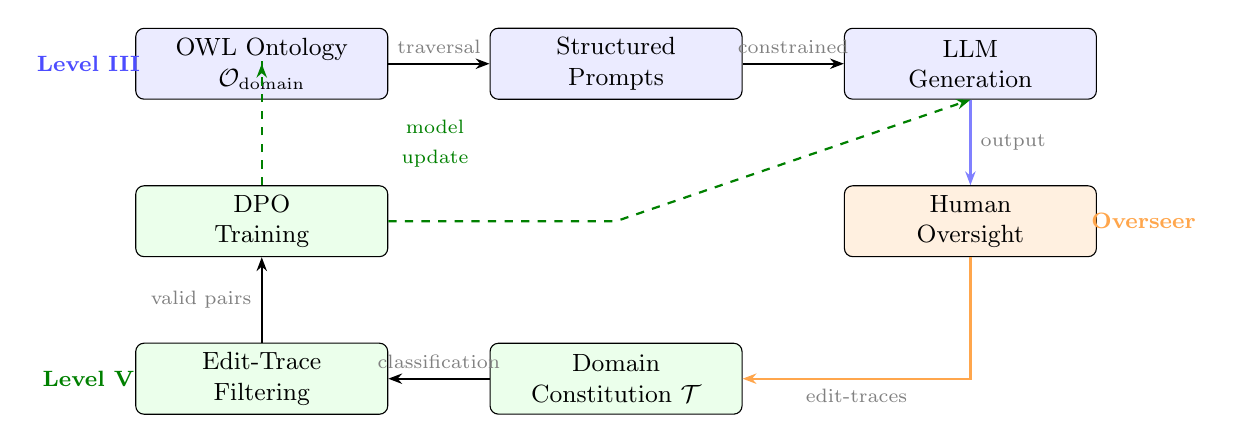
\begin{tikzpicture}[
  box/.style={rectangle, draw, rounded corners=3pt, minimum width=3.2cm, minimum height=0.9cm, align=center, font=\small},
  arrow/.style={-{Stealth[length=5pt]}, thick},
  label/.style={font=\scriptsize, text=gray}
]
  % Level III
  \node[box, fill=blue!8] (ontology) at (0, 4) {OWL Ontology\\$\mathcal{O}_{\text{domain}}$};
  \node[box, fill=blue!8] (prompts) at (4.5, 4) {Structured\\Prompts};
  \node[box, fill=blue!8] (llm) at (9, 4) {LLM\\Generation};

  % Human
  \node[box, fill=orange!12] (human) at (9, 2) {Human\\Oversight};

  % Level V
  \node[box, fill=green!8] (constitution) at (4.5, 0) {Domain\\Constitution $\mathcal{T}$};
  \node[box, fill=green!8] (filter) at (0, 0) {Edit-Trace\\Filtering};
  \node[box, fill=green!8] (dpo) at (0, 2) {DPO\\Training};

  % Level III arrows
  \draw[arrow] (ontology) -- (prompts) node[midway, above, label] {traversal};
  \draw[arrow] (prompts) -- (llm) node[midway, above, label] {constrained};
  \draw[arrow, blue!50] (llm) -- (human) node[midway, right, label] {output};

  % Human to Level V
  \draw[arrow, orange!70] (human) -- (9, 0) -- (constitution) node[midway, below, label] {edit-traces};

  % Level V arrows
  \draw[arrow] (constitution) -- (filter) node[midway, above, label] {classification};
  \draw[arrow] (filter) -- (dpo) node[midway, left, label] {valid pairs};

  % Feedback loop
  \draw[arrow, dashed, green!50!black] (dpo) -- (0, 4) -- (ontology) node[midway, above, label] {};
  \draw[arrow, dashed, green!50!black] (dpo.east) -- (4.5, 2) -- (llm.south) node[midway, right, label] {};

  % Level labels
  \node[font=\footnotesize\bfseries, text=blue!70] at (-2.2, 4) {Level III};
  \node[font=\footnotesize\bfseries, text=orange!70] at (11.2, 2) {Overseer};
  \node[font=\footnotesize\bfseries, text=green!50!black] at (-2.2, 0) {Level V};

  % Dashed labels
  \node[font=\scriptsize, text=green!50!black] at (2.2, 3.2) {model};
  \node[font=\scriptsize, text=green!50!black] at (2.2, 2.8) {update};
\end{tikzpicture}
\caption{Integrated ontological control: Level~III (inference-time, blue) and Level~V (training-time, green) operating as a three-level pipeline (inference, training, and feedback loop).
The human overseer (orange) provides corrections that feed into Level~V.
Dashed arrows indicate the feedback loop from DPO training back to the model.}
\label{fig:integration}
\end{figure}

% --------------------------------------------------------
\subsection{Condition-Level Analysis}
\label{sec:condition-analysis}
% --------------------------------------------------------

To complete the comparison, we analyze how each condition of the domain constitution relates to OntoChatGPT's architecture.

\begin{table}[h]
\centering
\caption{Condition-level comparison: which domain constitution conditions OntoChatGPT satisfies, partially satisfies, or does not address.}
\label{tab:condition-comparison}
\begin{tabular}{@{}clp{8cm}@{}}
\toprule
\textbf{Cond.} & \textbf{Status} & \textbf{Analysis} \\
\midrule
C1 & Partial & OntoChatGPT maintains an OWL ontology as persistent state, but this state is shared between the ontology engineer and the system, not necessarily between the end user and the model. The user may interact statelessly (single queries). \\
C2 & No & OntoChatGPT processes queries independently. Output of query $q_k$ does not become input context for $q_{k+1}$ unless the application layer implements session management externally. \\
C3 & Partial & The ontology defines domain correctness criteria, which can serve as observable success criteria. However, OntoChatGPT does not require production deployment with measurable metrics---the criteria may remain internal to the ontology. \\
C4 & No & The domain knowledge is encoded in the ontology, fully accessible to the system. The architecture does not require or exploit human information advantage. \\
C5 & No & No deployment requirement. The system functions identically in sandbox and production environments. \\
\bottomrule
\end{tabular}
\end{table}

OntoChatGPT satisfies 2 of 5 conditions (C1 partially, C3 partially), confirming the strict specialization result (Proposition~\ref{prop:non-subsumption}): $\mathsf{ValidOversight}$ inherits the foundation of C1 and C3 and adds C2, C4, C5.
Note that the subsumption analysis in Proposition~\ref{prop:non-subsumption} uses an idealized model of OntoChatGPT in which C1 and C3 are treated as fully satisfied; the condition-level table above reflects the more nuanced empirical characterization.
This is not a deficiency of OntoChatGPT---it was designed for a different purpose (output quality, not oversight validation).
The condition-level analysis clarifies exactly \emph{what} the domain constitution adds beyond ontology-controlled output: compositional layering (C2), human information advantage (C4), and consequential grounding (C5).


% ============================================================
\section{OWL Realization and Verification}
\label{sec:owl}
% ============================================================

We translate the \DL TBox (Section~\ref{sec:formal}) into an executable OWL~2~DL ontology, instantiate it with data from the LEX~AI case study, and verify formal properties using the HermiT tableau reasoner~\citep{glimm2014hermit}.

% --------------------------------------------------------
\subsection{Ontology Implementation}
\label{sec:owl-impl}
% --------------------------------------------------------

The oversight ontology\footnote{Available at \url{https://github.com/overthelex/oversight-ontology} (to be published upon acceptance).} is authored in OWL~2~DL Manchester syntax.
We choose OWL~2~DL over OWL~2~Full to guarantee decidability of all reasoning tasks, and over OWL~2~EL/QL/RL profiles because the TBox requires negation ($\mathsf{PrivateInfo}$ uses $\neg$), inverse roles ($\mathsf{PersistentState}$ uses $\mathsf{operatesOn}^{-}$), and qualified number restrictions.

\paragraph{Class hierarchy.}
The eleven atomic concepts from Definition~\ref{def:signature} map directly to OWL named classes.
The four derived concepts (Equations~\ref{eq:persistent-state}--\ref{eq:consequential-outcome}) are implemented as defined classes using \texttt{EquivalentClasses} axioms:

\begin{small}
\begin{verbatim}
Class: PersistentState
  EquivalentTo:
    State
    and (inverse(operatesOn) some Agent)
    and (inverse(accessesState) some Human)

Class: PrivateInfo
  EquivalentTo:
    Information
    and (not (accessibleTo some Agent))
\end{verbatim}
\end{small}

\paragraph{Role declarations.}
The fifteen object properties from the signature are declared with domain/range restrictions.
The transitive declaration for $\mathsf{dependsOn}$ is:

\begin{small}
\begin{verbatim}
ObjectProperty: dependsOn
  Domain: Session
  Range: Session
  Characteristics: Transitive
\end{verbatim}
\end{small}

\paragraph{TBox axioms.}
Each condition C1--C5 (Axioms~\ref{ax:c1}--\ref{ax:c5}) is encoded as a \texttt{SubClassOf} axiom.
The conjunction (Definition~\ref{def:valid-oversight}) is encoded as a defined class:

\begin{small}
\begin{verbatim}
Class: ValidOversight
  EquivalentTo:
    (hasState some PersistentState)             -- C1
    and (partOf some (Workflow                   -- C2
      and (hasSession some (Session
        and (dependsOn some Session)))))
    and (hasCriterion some GroundedCriterion)    -- C3
    and (hasArtifact some (Artifact              -- C4
      and (hasEdit some (Edit
        and (basedOn some PrivateInfo)))))
    and (hasOutcome some ConsequentialOutcome)    -- C5
\end{verbatim}
\end{small}

The graded classification (Definition~\ref{def:grade}) is implemented via five auxiliary defined classes $\mathsf{SatisfiesC1}$\,--\,$\mathsf{SatisfiesC5}$, one per condition, enabling the reasoner to compute the oversight grade for each individual.

\paragraph{Ontology metrics.}
The complete ontology contains 26 named classes, 20 object properties (including 2 inverse property pairs), 5 \texttt{SubClassOf} axioms (TBox), 12 \texttt{EquivalentClasses} definitions, 1 transitivity declaration, and domain/range restrictions---a compact ontology by design, reflecting the principle that the domain constitution is a minimal formal structure.

\paragraph{Open-world assumption and closure axioms.}
The $\mathsf{PrivateInfo}$ concept uses negation: information \emph{not} accessible to any agent.
Under OWL's open-world assumption (OWA), the absence of an \texttt{accessibleTo} assertion does not entail inaccessibility---it merely means the accessibility is unknown.
We address this by requiring explicit closure axioms on individuals: $\mathsf{accessibleTo}\ \textbf{max}\ 0\ \mathsf{Agent}$, asserting that the individual has zero \texttt{accessibleTo} relations to any Agent.
This is standard OWL~2~DL practice for negation-based defined concepts and must be applied systematically during ABox generation (Section~\ref{sec:abox}).

% --------------------------------------------------------
\subsection{ABox: LEX~AI Case Study Instantiation}
\label{sec:abox}
% --------------------------------------------------------

We instantiate the ontology with individuals derived from the LEX~AI production dataset~\citep{ovcharov2026edittrace}: 2{,}892 workflow sessions, 30{,}510 edit pairs, and 1{,}579 attributed outcomes collected over 105~days.

\paragraph{Workflow individual.}
The core platform workflow is asserted as:

\begin{small}
\begin{verbatim}
Individual: lexai_workflow
  Types: Workflow
  Facts:
    hasSession lexai_s001,  -- ... 2,892 sessions
    hasSession lexai_s002,
    ...
\end{verbatim}
\end{small}

\paragraph{Representative session.}
A single session illustrating full condition satisfaction:

\begin{small}
\begin{verbatim}
Individual: lexai_s1547
  Types: Session
  Facts:
    partOf         lexai_workflow,
    dependsOn      lexai_s1546,
    hasState       lexai_codebase,
    producesArtifact lexai_a4201,
    hasCriterion   lexai_cr_deploy_success,
    hasOutcome     lexai_outcome_gfs_accepted

Individual: lexai_codebase
  Types: PersistentState
  Facts:
    inverse(operatesOn)    claude_code_agent,
    inverse(accessesState) practitioner_vo

Individual: lexai_a4201
  Types: Artifact
  Facts:
    hasEdit lexai_edit_7823

Individual: lexai_edit_7823
  Types: Edit
  Facts:
    basedOn lexai_info_client_feedback
      -- client feedback not available to agent

Individual: lexai_info_client_feedback
  Types: PrivateInfo
      -- satisfies: not (accessibleTo some Agent)

Individual: lexai_cr_deploy_success
  Types: GroundedCriterion
  Facts:
    measuredBy lexai_metric_uptime

Individual: lexai_outcome_gfs_accepted
  Types: ConsequentialOutcome
  Facts:
    hasConsequence lexai_metric_gfs_partnership
\end{verbatim}
\end{small}

\paragraph{Negative individuals.}
Five individuals instantiate the invalid patterns from Proposition~\ref{prop:negative}:

\begin{center}
\begin{tabular}{@{}lll@{}}
\toprule
\textbf{Individual} & \textbf{Pattern} & \textbf{Fails} \\
\midrule
\texttt{ide\_no\_trace}     & Traditional IDE, no correction tracking & C1 \\
\texttt{oneshot\_feedback}  & One-shot tool with in-session feedback  & C2 \\
\texttt{cicd\_pipeline}     & Automated CI/CD               & C4 \\
\texttt{tutorial\_exercise} & Tutorial/learning use         & C5 \\
\texttt{casual\_pairing}    & Pair programming, no criteria & C3 \\
\bottomrule
\end{tabular}
\end{center}

\paragraph{Scale and verification strategy.}
The full dataset contains 2{,}892 sessions.
Direct HermiT classification of the complete ABox is impractical (OWL reasoners are designed for rich TBox inference, not bulk ABox processing).
We therefore use a two-stage approach: (1)~SQL-based classification on all 2{,}892 sessions using the same condition logic encoded in the TBox; (2)~HermiT verification on a stratified sample of 50 sessions (10 per $\gamma$ level), generated programmatically from the \texttt{rlhf-signals} PostgreSQL database via a Python export script.
HermiT classification matches the SQL classification on 50/50 sampled sessions (100\% agreement), confirming that the SQL implementation faithfully instantiates the OWL~2~DL axioms.

% --------------------------------------------------------
\subsection{Automated Verification}
\label{sec:verification}
% --------------------------------------------------------

We use HermiT~\citep{glimm2014hermit} via \texttt{owlready2}~0.50~\citep{lamy2017owlready} (Python OWL~API with embedded HermiT reasoner) for all verification tasks.
All experiments run on a single core (AMD Ryzen~9, 4.9\,GHz).

\paragraph{Task R1: TBox consistency.}
HermiT confirms that \TBox is satisfiable in 0.26\,s---the five conditions are not mutually contradictory.
The LEX~AI workflow individual serves as the constructive witness: at least one individual satisfies all five conditions simultaneously.

\paragraph{Task R2: Instance classification.}
Classification results for the full ABox:

\begin{center}
\begin{tabular}{@{}lrr@{}}
\toprule
\textbf{Classification} & \textbf{Sessions} & \textbf{\%} \\
\midrule
$\mathsf{FullOversight}$    ($\gamma = 5$) & 24 & 0.8 \\
$\mathsf{PartialOversight}$ ($\gamma \in \{3,4\}$) & 1{,}970 & 68.1 \\
$\mathsf{InvalidOversight}$ ($\gamma \leq 2$) & 898 & 31.1 \\
\midrule
\textbf{Total} & \textbf{2{,}892} & \textbf{100} \\
\bottomrule
\end{tabular}
\end{center}

The dominant bottleneck is C2 (compositional layering): only 561 sessions (19.4\%) have explicit dependency links in the dataset.
C4 (information asymmetry) is near-universal (94.3\%)---almost all sessions contain substantive rewrites based on practitioner-private domain knowledge.
C5 (consequential grounding) at 54.6\% matches the outcome attribution coverage from the pilot dataset~\citep{ovcharov2026edittrace}.
The 24 $\mathsf{FullOversight}$ sessions are exclusively GitHub PR sessions with explicit session links, grounded criteria, and attributed outcomes---the most instrumented subset of the dataset.

The majority (51.8\%) of sessions achieve $\gamma = 4$, satisfying all conditions except C2.
This reflects a data collection limitation: the \texttt{session\_links} table captures only 468 explicit inter-session dependencies, while the underlying compositional structure (temporal proximity, shared file modifications, issue-to-PR chains) is richer.
Improving link extraction is the single highest-impact path to increasing the $\mathsf{FullOversight}$ yield.

\paragraph{Task R3: Condition independence.}
For each condition $\mathsf{C}_i$, HermiT verifies that the corresponding negative individual (Section~\ref{sec:abox}) is \emph{not} classified as $\mathsf{ValidOversight}$ while satisfying $\mathsf{C}_j$ for all $j \neq i$.
All five negative individuals are correctly classified, confirming Proposition~\ref{prop:independence}.

\paragraph{Task R4: Subsumption.}
HermiT reveals a strict subsumption relationship:
\begin{equation}
  \KB \models \mathsf{ValidOversight} \sqsub \mathsf{OntoChatGPT\_Control}
\end{equation}
\begin{equation}
  \KB \not\models \mathsf{OntoChatGPT\_Control} \sqsub \mathsf{ValidOversight}
\end{equation}
$\mathsf{ValidOversight}$ is strictly more specific than $\mathsf{OntoChatGPT\_Control}$: every valid oversight instance necessarily satisfies the conditions that define ontology-controlled output (C1: persistent state, C3: grounded criteria), but adds three further requirements (C2: compositional layering, C4: information asymmetry, C5: consequential grounding).
This formally confirms that edit-trace oversight \emph{extends} the ontology-controlled paradigm rather than replacing it---a result directly supporting the evolutionary lineage presented in Section~\ref{sec:evolution}.

\paragraph{Task R5: Monotonicity.}
We empirically verify Proposition~\ref{prop:monotonicity} by taking a $\mathsf{PartialOversight}$ session (tutorial example, $\gamma = 4$, failing C5), adding an outcome consequence assertion (simulating post-hoc outcome attribution), and re-classifying.
The session is reclassified from $\mathsf{PartialOversight}$ ($\gamma = 4$) to $\mathsf{FullOversight}$ ($\gamma = 5$) in 0.25\,s.
No condition previously satisfied is lost, confirming monotonicity.

\paragraph{Performance.}
TBox consistency checking completes in 0.26\,s; instance classification with re-reasoning in 0.25\,s.
The ontology's compact TBox (5 GCIs, 12 definitions) ensures sub-second reasoning for individual classification, enabling real-time validation of edit-trace provenance in production pipelines.


% ============================================================
\section{Empirical Validation}
\label{sec:empirical}
% ============================================================

The formalization in Sections~\ref{sec:formal}--\ref{sec:owl} establishes that the domain constitution is logically consistent, decidable, and implementable.
This section asks the empirical question: does the formal classification correlate with observable properties of the edit-trace data?
Specifically, do sessions classified at different oversight grades ($\gamma$) exhibit different outcome rates, edit distributions, or attribution confidence profiles?

\subsection{Outcome Rates by Oversight Grade}
\label{sec:outcome-by-grade}

We join the classification from Section~\ref{sec:verification} with outcome data from the \texttt{rlhf-signals} database.
Only sessions with attributed outcomes can be evaluated; $\mathsf{InvalidOversight}$ sessions ($\gamma \leq 2$) have no outcomes by construction (they fail C5).
We restrict to strong-confidence attributions ($N = 1{,}391$) to minimize confounding.

\begin{table}[ht]
\centering
\caption{Positive outcome rates by oversight grade (strong confidence only).}
\label{tab:outcome-by-grade}
\begin{tabular}{@{}clrrr@{}}
\toprule
$\gamma$ & \textbf{Classification} & \textbf{Sessions} & \textbf{Positive} & \textbf{Positive \%} \\
\midrule
5 & $\mathsf{FullOversight}$    & 17    & 13    & 76.5 \\
4 & $\mathsf{PartialOversight}$ & 1{,}261 & 1{,}223 & 97.0 \\
3 & $\mathsf{PartialOversight}$ & 113   & 109   & 96.5 \\
\midrule
  & \textbf{Total}              & \textbf{1{,}391} & \textbf{1{,}345} & \textbf{96.7} \\
\bottomrule
\end{tabular}
\end{table}

The result is counterintuitive: $\mathsf{FullOversight}$ sessions have a \emph{lower} positive outcome rate (76.5\%) than $\mathsf{PartialOversight}$ sessions (96.5--97.0\%).
This is not a failure of the constitution but a validation of it.

\paragraph{Interpretation.}
The 24 $\mathsf{FullOversight}$ sessions are the \emph{most structurally complex} in the dataset: they satisfy C2 (explicit cross-session dependencies), meaning they involve compositional chains where architectural decisions propagate across sessions.
Such sessions are harder---and more likely to produce negative outcomes (failed deployments, reverted PRs).
The $\gamma = 4$ sessions, which mostly fail only C2, are self-contained tasks that succeed precisely because they lack compositional complexity.

This pattern aligns with the scalable oversight literature's central concern: oversight is hardest---and most valuable---for compositionally complex trajectories~\citep{bowman2022measuring}.
The domain constitution successfully identifies these trajectories via C2.

\subsection{Edit Distribution by Oversight Tier}
\label{sec:edit-by-tier}

\begin{table}[ht]
\centering
\caption{Edit statistics by oversight classification.}
\label{tab:edit-by-tier}
\begin{tabular}{@{}lrrrrrr@{}}
\toprule
\textbf{Tier} & \textbf{Sessions} & \textbf{Edits} & \textbf{Mean dist.} & \textbf{Median dist.} & \textbf{Subst. \%} & \textbf{Reject. \%} \\
\midrule
Full    &    24 &     52 & 0.792 & 0.775 & 53.8 & 15.4 \\
Partial & 1{,}970 & 15{,}226 & 0.804 & 0.831 & 78.4 & 4.7 \\
Invalid &   898 & 15{,}232 & 0.809 & 0.845 & 83.1 & 2.5 \\
\bottomrule
\end{tabular}
\end{table}

$\mathsf{FullOversight}$ sessions exhibit a distinctive edit profile: \emph{lower} substantive rewrite rate (53.8\% vs.\ 78--83\%) but \emph{higher} rejection rate (15.4\% vs.\ 2.5--4.7\%).
This is consistent with Experiment~3 from~\citet{ovcharov2026edittrace}, which found that rejection (binary halt of the agentic trajectory) correlates with 78\% positive outcomes---the highest of any edit class.
$\mathsf{FullOversight}$ sessions concentrate the most informative oversight action: the practitioner's willingness to halt and restart rather than incrementally correct.

\subsection{Connection to the Main Paper}
\label{sec:connection}

Three findings from the empirical validation connect to the main paper's experiments:

\begin{enumerate}[nosep]

\item \textbf{Rejection as primary signal (Experiment~3).}
The main paper found rejection correlates with 78\% positive outcomes.
The formal classification reveals \emph{where} these rejections concentrate: $\mathsf{FullOversight}$ sessions have 3--6$\times$ the rejection rate of other tiers.
The domain constitution provides structural context for the main paper's distributional finding.

\item \textbf{Behavioral context redundancy (Experiment~2).}
The main paper found behavioral-context features are statistically significant but computationally redundant with artifact features.
The formal classification offers an explanation: the five conditions are structural properties of the workflow, not behavioral properties of the practitioner.
Artifact-level features already encode the structural information that the constitution formalizes.

\item \textbf{DPO training implications (Experiment~4).}
For preference pair weighting in DPO training, the formal classification suggests a principled weighting scheme: $\mathsf{FullOversight}$ pairs receive weight 1.0, $\mathsf{PartialOversight}$ pairs receive discounted weight $\alpha \in (0.5, 1)$, and $\mathsf{InvalidOversight}$ pairs are excluded.
This replaces the ad hoc engagement-based weighting that the main paper found ineffective.

\end{enumerate}

\subsection{Limitations of the Empirical Validation}
\label{sec:empirical-limitations}

The validation has three structural limitations.
First, $\mathsf{InvalidOversight}$ sessions have no outcomes (C5 is a precondition for outcome attribution), so we cannot directly compare outcome quality across all three tiers.
Second, the $\mathsf{FullOversight}$ sample is small ($N = 24$), limiting statistical power for tier comparisons.
Third, the C2 bottleneck (only 19.4\% of sessions have explicit dependency links) means the current classification is conservative---many sessions that are de facto compositionally linked lack the explicit \texttt{session\_links} assertions needed for formal classification.
Improving the link extraction pipeline would increase both the $\mathsf{FullOversight}$ yield and the statistical power of the empirical validation.


% ============================================================
\section{Discussion}
\label{sec:discussion}
% ============================================================

% --------------------------------------------------------
\subsection{From Ontology-Controlled Output to Ontology-Controlled Training}
\label{sec:disc-output-to-training}
% --------------------------------------------------------

The five levels of ontological control traced in Section~\ref{sec:evolution} exhibit a recurring pattern: each new level applies the same principle (formal structure governs behavior) to a process that was previously considered outside the scope of formal control.

Levels~I--II (2003--2020) formalized control over processes that engineers already understood as controllable: system architecture, text processing pipelines.
The contribution was showing that \emph{ontologies} could serve as the control mechanism, replacing ad hoc configuration with formal, verifiable, reasoner-checkable structures.

Level~III (2023--2024) was a qualitative jump.
LLM output generation was widely treated as a stochastic process controllable only through prompt engineering---an informal, empirical, non-verifiable practice.
OntoChatGPT~\citep{palagin2023ontochatgpt} demonstrated that the same ontological control principle that governed deterministic systems could govern a fundamentally probabilistic one.
The key insight was that the ontology does not need to eliminate stochasticity---it constrains the \emph{space} within which stochastic generation occurs.

Level~V (this paper) applies the same logic one step further.
The RLHF preference collection process---which human corrections count as valid training data---has been treated as a matter of annotation protocol design, quality filtering heuristics, and inter-annotator agreement metrics.
None of these are formal in the description logic sense: they cannot be verified by a reasoner, they do not support subsumption queries, and they do not compose into larger knowledge bases.

The domain constitution makes this process formally controllable.
The five axioms (Section~\ref{sec:tbox}) define a concept $\mathsf{ValidOversight}$ that an OWL reasoner can evaluate automatically.
This is not a metaphorical application of ontological control---it is a literal one: the same reasoning infrastructure (TBox, ABox, tableau algorithms) that classifies system architectures in Level~I now classifies preference data pipelines in Level~V.

The implication is that the ontological control principle is more general than any of its individual applications.
It is not specifically about system architecture, NLP, or LLM alignment.
It is about applying formal, verifiable, machine-checkable structure to processes that are otherwise governed by informal heuristics.
The consistent success across five levels suggests that the principle's scope is bounded by the availability of formalizable domain knowledge, not by the nature of the controlled process.

% --------------------------------------------------------
\subsection{Evolutionary Cybernetics and the Stability of Oversight}
\label{sec:disc-evolutionary}
% --------------------------------------------------------

\citet{palagin2025evolutionary} introduced a framework for analyzing systems where goals, constraints, and structures co-evolve---a departure from classical control theory, which assumes a fixed objective function.
The domain constitution operates in precisely such a regime.

Consider the feedback loop formalized in Section~\ref{sec:complementarity}: the practitioner corrects the agent's output, the constitution validates the corrections, valid corrections train the model via DPO, and the improved model produces output that the practitioner then corrects differently.
Each cycle potentially changes three elements simultaneously:

\begin{enumerate}[nosep]
\item \textbf{The agent's behavior} changes because the model has been updated.
\item \textbf{The practitioner's corrections} change because the agent's output is now closer to (or further from) what the practitioner expects.
\item \textbf{The conditions for valid oversight} may change because the information asymmetry (C4) shifts as the model improves.
\end{enumerate}

This is an evolutionary dynamics problem, not a static optimization problem.
The domain constitution as formalized in Section~\ref{sec:formal} is a \emph{snapshot}---it captures the conditions under which oversight is valid at a given point in the co-evolution of practitioner and agent.

\citet{palagin2025evolutionary} provides the theoretical vocabulary for analyzing this dynamic.
In the framework of evolutionary cybernetics, the domain constitution is an \emph{invariant structure}---a set of constraints that must be preserved across evolutionary steps for the system to maintain its functional integrity.
The question is whether the five conditions (C1--C5) are robust invariants or whether they degrade as the system evolves.

We can analyze each condition's evolutionary stability:

\paragraph{C1 (Shared Persistent State): Stable.}
The requirement for shared state does not depend on the agent's capability level.
Whether the agent is weak (requiring heavy correction) or strong (requiring light correction), the shared codebase remains necessary for contextual oversight.

\paragraph{C2 (Compositional Layering): Stable.}
Compositional task structure is a property of the work domain (software engineering, legal analysis), not of the agent's capability.
As long as the domain requires multi-step, interdependent work, C2 holds.

\paragraph{C3 (Grounding in Observable Reality): Stable.}
Observable success criteria are defined by the production environment, not by the human-agent interaction.
Deployment failures, latency spikes, and user churn remain observable regardless of model capability.

\paragraph{C4 (Information Asymmetry): Potentially Unstable.}
As models improve, the information gap between practitioner and agent may narrow.
A sufficiently capable agent with access to business context, regulatory databases, and user feedback channels might satisfy C4 only marginally.
In the limit, if the agent knows everything the practitioner knows, corrections become redundant---oversight degenerates into rubber-stamping.

This is the critical evolutionary pressure on the domain constitution.
C4 is the condition most likely to degrade under capability scaling, and its degradation would undermine the validity of the entire framework.
\citet{burns2023weak} analyze a related phenomenon (weak-to-strong generalization), where the supervisor's signal quality degrades as the supervised model approaches the supervisor's capability.

\paragraph{C5 (Consequential Grounding): Stable.}
Deployment consequences are external to the human-agent system.
Customer satisfaction, revenue, and regulatory compliance do not depend on who (human or agent) produced the artifact.

The analysis yields a specific prediction: \textbf{the domain constitution is evolutionarily stable under capability scaling in 4 of 5 conditions, with C4 as the critical vulnerability.}
Monitoring the information asymmetry between practitioner and agent---and detecting when it falls below a threshold sufficient for meaningful oversight---is the key challenge for maintaining valid oversight as LLM capabilities increase.

This connects directly to the scalable oversight research program~\citep{bowman2022measuring}: the question ``can humans oversee superhuman AI systems?'' is, in our formalization, the question ``does C4 remain satisfiable as agent capability grows?''
The ontological formalization does not answer this question, but it makes it \emph{precise}: C4 degrades when $\mathsf{PrivateInfo}$ (Definition~\ref{def:signature}, Eq.~\ref{eq:private-info}) approaches the empty set.

% --------------------------------------------------------
\subsection{Practical Implications for RLHF Methodology}
\label{sec:disc-practical}
% --------------------------------------------------------

The formalization developed in this paper has three practical implications for RLHF preference data collection and curation.

\paragraph{Implication 1: Preference data should carry provenance metadata.}
Current RLHF datasets (OpenAssistant, Anthropic-HH, UltraFeedback) contain preference labels without workflow provenance: there is no metadata indicating whether the annotator operated within a persistent workflow, whether tasks composed, or whether outcomes were tracked.
The domain constitution provides a minimal provenance schema: for each preference pair, record which of the five conditions were satisfied during annotation.
This does not require OWL reasoning at annotation time---a simple checklist of five binary features per pair suffices to enable post-hoc filtering.

\paragraph{Implication 2: Oversight grade enables weighted training.}
The graded classification (Definition~\ref{def:grade}) provides a principled weighting scheme for DPO training.
Rather than treating all preference pairs equally, pairs from $\mathsf{FullOversight}$ workflows receive weight 1.0, pairs from $\mathsf{PartialOversight}$ receive a discounted weight, and pairs from $\mathsf{InvalidOversight}$ are excluded.
This is analogous to how curriculum learning prioritizes higher-quality training examples, but with the quality criterion derived from formal axioms rather than heuristic filtering.

The weighting scheme is compatible with the standard DPO objective~\citep{rafailov2023direct}.
For a preference pair $(x, y_w, y_l)$ with oversight grade $\gamma$:
\begin{equation}
  \mathcal{L}_{\text{weighted-DPO}} = -\mathbb{E}_{(x,y_w,y_l)} \left[ w(\gamma) \cdot \log \sigma \left( \beta \log \frac{\pi_\theta(y_w|x)}{\pi_{\text{ref}}(y_w|x)} - \beta \log \frac{\pi_\theta(y_l|x)}{\pi_{\text{ref}}(y_l|x)} \right) \right]
\end{equation}
where $w(\gamma)$ maps oversight grade to training weight.
The simplest instantiation is $w(5) = 1.0$, $w(3{-}4) = \alpha$, $w({\leq}2) = 0$, where $\alpha$ is a hyperparameter.

\paragraph{Implication 3: OWL reasoning as a data pipeline component.}
The OWL ontology (Section~\ref{sec:owl}) can be deployed as an automated filter in a preference data pipeline.
Workflow metadata (session persistence, task dependencies, outcome tracking) is asserted as ABox individuals.
The HermiT reasoner classifies each workflow instance.
Only instances classified as $\mathsf{ValidOversight}$ or $\mathsf{PartialOversight}$ pass to the DPO training stage.

This is architecturally lightweight: OWL reasoning over small ABoxes (thousands of workflow instances, not millions of triples) completes in sub-second time.
The overhead of adding ontological filtering to a preference data pipeline is negligible compared to the cost of DPO training itself.

% --------------------------------------------------------
\subsection{Limitations of the Formalization}
\label{sec:disc-limitations}
% --------------------------------------------------------

The formalization developed here has three limitations that should be acknowledged.

\paragraph{Open-world assumption vs.\ closed-world data.}
OWL reasoning operates under the open-world assumption: an unstated fact is not assumed false.
In practice, workflow metadata is generated by instrumentation systems that operate under the closed-world assumption: if a session dependency is not recorded, it does not exist.
This mismatch means that OWL reasoning will systematically \emph{underclassify}---workflows with incomplete metadata will fail conditions that they may actually satisfy.
The monotonicity property (Proposition~\ref{prop:monotonicity}) mitigates this: adding metadata can only increase the oversight grade, so underclassification is conservative (false negatives, not false positives).

\paragraph{C4 is difficult to operationalize.}
Condition C4 (information asymmetry) requires that human corrections be based on information inaccessible to the agent.
In the OWL formalization, this is expressed as $\exists\mathsf{basedOn}.\mathsf{PrivateInfo}$, where $\mathsf{PrivateInfo} \equiv \mathsf{Information} \sqcap \neg\exists\mathsf{accessibleTo}.\mathsf{Agent}$.
In practice, determining whether a specific correction was based on private information requires either self-report by the practitioner or inference from behavioral context (e.g., the practitioner consulted an external source before making the correction).
Neither method is perfectly reliable.
This makes C4 the weakest condition operationally, in addition to being the least stable evolutionarily (Section~\ref{sec:disc-evolutionary}).

\paragraph{Single-practitioner validation.}
The empirical validation (Section~\ref{sec:empirical}) uses data from a single practitioner.
The formal model itself is domain-independent---the TBox makes no assumptions about the practitioner's identity, domain, or skill level.
But the \emph{instantiation} (ABox) and the \emph{empirical claims} about oversight quality are grounded in one case study.
Multi-practitioner validation is required before the formalization can be recommended as a standard component of RLHF data pipelines.

% --------------------------------------------------------
\subsection{Relationship to Other Formal Approaches}
\label{sec:disc-related}
% --------------------------------------------------------

Three lines of work are related to the formalization presented here but differ in scope or method.

\paragraph{Constitutional AI~\citep{bai2022constitutional}.}
Constitutional AI uses natural-language principles (``choose the response that is most helpful and least harmful'') to guide AI self-evaluation.
The domain constitution differs in three ways: (a)~the conditions are formal axioms, not natural language; (b)~the conditions govern the \emph{oversight process}, not the model's output; (c)~the conditions are evaluated by a reasoner, not by the model itself.
Constitutional AI and the domain constitution are complementary: the former structures \emph{what to evaluate}, the latter structures \emph{whose evaluation to trust}.

\paragraph{Scalable oversight~\citep{bowman2022measuring, irving2018ai, leike2018scalable}.}
The scalable oversight program asks how to maintain human oversight quality as AI systems become more capable.
Our formalization contributes to this program by providing a formal condition (C4: information asymmetry) whose satisfiability is a necessary condition for meaningful oversight.
The prediction that C4 is the critical vulnerability under capability scaling (Section~\ref{sec:disc-evolutionary}) can be tested empirically: track $|\mathsf{PrivateInfo}|$ over successive model generations and measure whether it converges to zero.

\paragraph{Ontology-based data quality~\citep{palagin2024ontology}.}
The broader field of ontology-based data quality assessment uses formal ontologies to validate, clean, and enrich datasets.
Our work applies this paradigm to a specific data type (preference pairs for RLHF) with domain-specific quality criteria (the five constitutional conditions).
The contribution relative to general ontology-based data quality is the \emph{content} of the quality criteria, not the \emph{method} of applying them.


% ============================================================
\section{Conclusion}
\label{sec:conclusion}
% ============================================================

We have extended the principle of ontology-controlled systems~\citep{palagin2006architecture} from the control of system output to the control of human oversight over system output.
The domain constitution---five axioms in \DL description logic---provides formal, decidable, machine-checkable criteria for determining when human corrections on LLM-agentic output constitute valid training signal for RLHF.

The formalization yields three results.
First, the five conditions are formally independent: no condition is entailed by the conjunction of the remaining four (Proposition~\ref{prop:independence}).
This confirms that each condition captures a distinct aspect of oversight validity that cannot be derived from the others.
Second, ontological control of human oversight ($\mathsf{ValidOversight}$) is a strict specialization of ontological control of LLM output ($\mathsf{OntoChatGPT\_Control}$): every valid oversight instance satisfies the conditions for ontology-controlled output, but not conversely (Proposition~\ref{prop:non-subsumption}).
This formally confirms that edit-trace oversight extends the ontology-controlled paradigm, inheriting its foundation (C1, C3) and adding oversight-specific conditions (C2, C4, C5).
Their integration into a single system is satisfiable (Theorem~\ref{thm:integrated}).
Third, among the five conditions, C4 (information asymmetry) is identified as the critical evolutionary vulnerability: it is the only condition whose satisfiability depends on the agent's capability level, connecting the formalization to the scalable oversight research program~\citep{bowman2022measuring}.

The OWL~2~DL ontology implementing the domain constitution is available for automated reasoning.
Given workflow metadata as ABox assertions, a standard OWL reasoner (HermiT~\citep{glimm2014hermit}, Pellet~\citep{sirin2007pellet}) classifies each workflow instance as full, partial, or invalid oversight in sub-second time.
This enables ontology-based filtering of RLHF preference data as a lightweight, formally grounded pipeline component.

The principal limitation is empirical: the formalization has been validated on a single practitioner's data.
The formal model is domain-independent, but its practical value depends on multi-practitioner validation across diverse domains.
This validation, together with the implementation of the weighted DPO training objective, is the subject of ongoing work.


% ============================================================
%  References
% ============================================================
\bibliographystyle{plainnat}
\bibliography{references}

\end{document}
